\documentclass[border=3pt,tikz]{standalone}
\usepackage{pgfplots}

\usetikzlibrary{arrows}
\usetikzlibrary{shadows}
\usetikzlibrary{positioning}
\usetikzlibrary{calc}
\usetikzlibrary{patterns}


\tikzstyle{block} = [draw,rectangle,thick,minimum height=2em,minimum width=2em,drop shadow,fill=green!40!white]
\tikzstyle{sum} = [draw,circle,inner sep=0mm,minimum size=2mm]
\tikzstyle{terminal} = [draw,circle,inner sep=0mm,minimum size=1.5mm]
\tikzstyle{connector} = [->,thick]
\tikzstyle{line} = [very thick]
\tikzstyle{branch} = [circle,inner sep=0pt,minimum size=1mm,fill=black,draw=black]
\tikzstyle{axes} = [->,>=stealth',semithick]
\tikzstyle{important line} = [very thick,draw=red]
\tikzstyle{important text} = [rounded corners,fill=red!10,inner sep=1ex]
\pgfplotsset{compat=1.18}

\begin{document}

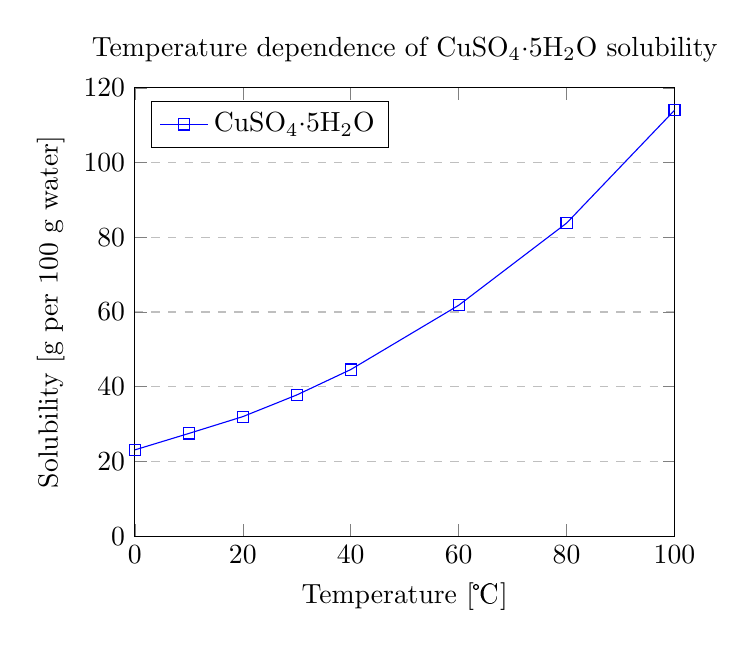
\begin{tikzpicture}
    \begin{axis}[
        title={Temperature dependence of CuSO\(_4\cdot\)5H\(_2\)O solubility},
        xlabel={Temperature [\textcelsius]},
        ylabel={Solubility [g per 100 g water]},
        xmin=0, xmax=100,
        ymin=0, ymax=120,
        xtick={0,20,40,60,80,100},
        ytick={0,20,40,60,80,100,120},
        legend pos=north west,
        ymajorgrids=true,
        grid style=dashed,
    ]
    
    \addplot[
        color=blue,
        mark=square,
        ]
        coordinates {
        (0,23.1)(10,27.5)(20,32)(30,37.8)(40,44.6)(60,61.8)(80,83.8)(100,114)
        };
        \legend{CuSO\(_4\cdot\)5H\(_2\)O}
        
    \end{axis}
\end{tikzpicture}

\end{document}